% Options for packages loaded elsewhere
\PassOptionsToPackage{unicode}{hyperref}
\PassOptionsToPackage{hyphens}{url}
%
\documentclass[
]{article}
\usepackage{amsmath,amssymb}
\usepackage{iftex}
\ifPDFTeX
  \usepackage[T1]{fontenc}
  \usepackage[utf8]{inputenc}
  \usepackage{textcomp} % provide euro and other symbols
\else % if luatex or xetex
  \usepackage{unicode-math} % this also loads fontspec
  \defaultfontfeatures{Scale=MatchLowercase}
  \defaultfontfeatures[\rmfamily]{Ligatures=TeX,Scale=1}
\fi
\usepackage{lmodern}
\ifPDFTeX\else
  % xetex/luatex font selection
\fi
% Use upquote if available, for straight quotes in verbatim environments
\IfFileExists{upquote.sty}{\usepackage{upquote}}{}
\IfFileExists{microtype.sty}{% use microtype if available
  \usepackage[]{microtype}
  \UseMicrotypeSet[protrusion]{basicmath} % disable protrusion for tt fonts
}{}
\makeatletter
\@ifundefined{KOMAClassName}{% if non-KOMA class
  \IfFileExists{parskip.sty}{%
    \usepackage{parskip}
  }{% else
    \setlength{\parindent}{0pt}
    \setlength{\parskip}{6pt plus 2pt minus 1pt}}
}{% if KOMA class
  \KOMAoptions{parskip=half}}
\makeatother
\usepackage{xcolor}
\usepackage[margin=1in]{geometry}
\usepackage{color}
\usepackage{fancyvrb}
\newcommand{\VerbBar}{|}
\newcommand{\VERB}{\Verb[commandchars=\\\{\}]}
\DefineVerbatimEnvironment{Highlighting}{Verbatim}{commandchars=\\\{\}}
% Add ',fontsize=\small' for more characters per line
\usepackage{framed}
\definecolor{shadecolor}{RGB}{248,248,248}
\newenvironment{Shaded}{\begin{snugshade}}{\end{snugshade}}
\newcommand{\AlertTok}[1]{\textcolor[rgb]{0.94,0.16,0.16}{#1}}
\newcommand{\AnnotationTok}[1]{\textcolor[rgb]{0.56,0.35,0.01}{\textbf{\textit{#1}}}}
\newcommand{\AttributeTok}[1]{\textcolor[rgb]{0.13,0.29,0.53}{#1}}
\newcommand{\BaseNTok}[1]{\textcolor[rgb]{0.00,0.00,0.81}{#1}}
\newcommand{\BuiltInTok}[1]{#1}
\newcommand{\CharTok}[1]{\textcolor[rgb]{0.31,0.60,0.02}{#1}}
\newcommand{\CommentTok}[1]{\textcolor[rgb]{0.56,0.35,0.01}{\textit{#1}}}
\newcommand{\CommentVarTok}[1]{\textcolor[rgb]{0.56,0.35,0.01}{\textbf{\textit{#1}}}}
\newcommand{\ConstantTok}[1]{\textcolor[rgb]{0.56,0.35,0.01}{#1}}
\newcommand{\ControlFlowTok}[1]{\textcolor[rgb]{0.13,0.29,0.53}{\textbf{#1}}}
\newcommand{\DataTypeTok}[1]{\textcolor[rgb]{0.13,0.29,0.53}{#1}}
\newcommand{\DecValTok}[1]{\textcolor[rgb]{0.00,0.00,0.81}{#1}}
\newcommand{\DocumentationTok}[1]{\textcolor[rgb]{0.56,0.35,0.01}{\textbf{\textit{#1}}}}
\newcommand{\ErrorTok}[1]{\textcolor[rgb]{0.64,0.00,0.00}{\textbf{#1}}}
\newcommand{\ExtensionTok}[1]{#1}
\newcommand{\FloatTok}[1]{\textcolor[rgb]{0.00,0.00,0.81}{#1}}
\newcommand{\FunctionTok}[1]{\textcolor[rgb]{0.13,0.29,0.53}{\textbf{#1}}}
\newcommand{\ImportTok}[1]{#1}
\newcommand{\InformationTok}[1]{\textcolor[rgb]{0.56,0.35,0.01}{\textbf{\textit{#1}}}}
\newcommand{\KeywordTok}[1]{\textcolor[rgb]{0.13,0.29,0.53}{\textbf{#1}}}
\newcommand{\NormalTok}[1]{#1}
\newcommand{\OperatorTok}[1]{\textcolor[rgb]{0.81,0.36,0.00}{\textbf{#1}}}
\newcommand{\OtherTok}[1]{\textcolor[rgb]{0.56,0.35,0.01}{#1}}
\newcommand{\PreprocessorTok}[1]{\textcolor[rgb]{0.56,0.35,0.01}{\textit{#1}}}
\newcommand{\RegionMarkerTok}[1]{#1}
\newcommand{\SpecialCharTok}[1]{\textcolor[rgb]{0.81,0.36,0.00}{\textbf{#1}}}
\newcommand{\SpecialStringTok}[1]{\textcolor[rgb]{0.31,0.60,0.02}{#1}}
\newcommand{\StringTok}[1]{\textcolor[rgb]{0.31,0.60,0.02}{#1}}
\newcommand{\VariableTok}[1]{\textcolor[rgb]{0.00,0.00,0.00}{#1}}
\newcommand{\VerbatimStringTok}[1]{\textcolor[rgb]{0.31,0.60,0.02}{#1}}
\newcommand{\WarningTok}[1]{\textcolor[rgb]{0.56,0.35,0.01}{\textbf{\textit{#1}}}}
\usepackage{graphicx}
\makeatletter
\def\maxwidth{\ifdim\Gin@nat@width>\linewidth\linewidth\else\Gin@nat@width\fi}
\def\maxheight{\ifdim\Gin@nat@height>\textheight\textheight\else\Gin@nat@height\fi}
\makeatother
% Scale images if necessary, so that they will not overflow the page
% margins by default, and it is still possible to overwrite the defaults
% using explicit options in \includegraphics[width, height, ...]{}
\setkeys{Gin}{width=\maxwidth,height=\maxheight,keepaspectratio}
% Set default figure placement to htbp
\makeatletter
\def\fps@figure{htbp}
\makeatother
\setlength{\emergencystretch}{3em} % prevent overfull lines
\providecommand{\tightlist}{%
  \setlength{\itemsep}{0pt}\setlength{\parskip}{0pt}}
\setcounter{secnumdepth}{-\maxdimen} % remove section numbering
\usepackage{fontspec}
\setmainfont{Arial}
\ifLuaTeX
  \usepackage{selnolig}  % disable illegal ligatures
\fi
\IfFileExists{bookmark.sty}{\usepackage{bookmark}}{\usepackage{hyperref}}
\IfFileExists{xurl.sty}{\usepackage{xurl}}{} % add URL line breaks if available
\urlstyle{same}
\hypersetup{
  hidelinks,
  pdfcreator={LaTeX via pandoc}}

\author{}
\date{\vspace{-2.5em}}

\begin{document}

\hypertarget{universidade-federal-do-paranuxe1}{%
\section{UNIVERSIDADE FEDERAL DO
PARANÁ}\label{universidade-federal-do-paranuxe1}}

PPGECon\\
Disciplina: Estatística\\
Professor: Adalto Acir Althaus Junior

\hypertarget{lista-de-exercuxedcios-01}{%
\section{Lista de Exercícios 01}\label{lista-de-exercuxedcios-01}}

\hypertarget{item-1-dataset-1}{%
\subsection{Item 1 (dataset 1)}\label{item-1-dataset-1}}

A planilha DEMO traz informações de 1.000 respondentes quanto à sua
idade em anos, o seu estado civil (1- casado , 0- não casado), quanto
tempo (em anos) vive no endereço atual, sua renda anual (em milhares de
reais), o preço do carro principal (em milhares de reais), sua
escolaridade (1- primeiro grau, 2- segundo grau, 3- terceiro grau, 4-
Pós graduação especialização, 5- mestrado/doutorado), quanto tempo, em
anos, está no emprego atual (t\_emp\_atual), se é (1) ou não (0)
aposentado, o sexo (m- masc e f- femin) e sua satisfação no trabalho (de
1- Nada satisfeito a 5- Muito satisfeito).

\hypertarget{apurauxe7uxe3o}{%
\subsubsection{APURAÇÃO}\label{apurauxe7uxe3o}}

\begin{Shaded}
\begin{Highlighting}[]
\NormalTok{df1 }\OtherTok{\textless{}{-}} \FunctionTok{read\_csv2}\NormalTok{(}\StringTok{"C:/Users/DELL/OneDrive/R/Rprojetos/ufpr\_ppgecon/estatistica/data/Exerc\_1\_descritiva\_dataset1.csv"}\NormalTok{)}
\end{Highlighting}
\end{Shaded}

\begin{verbatim}
## i Using "','" as decimal and "'.'" as grouping mark. Use `read_delim()` for more control.
\end{verbatim}

\begin{verbatim}
## Rows: 1000 Columns: 10
## -- Column specification -------------------------------------------------------------------------------------------------------------------------------
## Delimiter: ";"
## chr (1): sexo
## dbl (9): idade, est_civil, endereco, renda, carro, escolaridade, t_empr_atual, aposentado, satisf_trabal
## 
## i Use `spec()` to retrieve the full column specification for this data.
## i Specify the column types or set `show_col_types = FALSE` to quiet this message.
\end{verbatim}

\begin{Shaded}
\begin{Highlighting}[]
\NormalTok{df1}
\end{Highlighting}
\end{Shaded}

\begin{verbatim}
## # A tibble: 1,000 x 10
##    idade est_civil endereco renda carro escolaridade t_empr_atual aposentado satisf_trabal sexo 
##    <dbl>     <dbl>    <dbl> <dbl> <dbl>        <dbl>        <dbl>      <dbl>         <dbl> <chr>
##  1    55         1       12    72  36.2            1           23          0             5 f    
##  2    56         0       29   153  76.9            1           35          0             4 m    
##  3    28         1        9    28  13.7            3            4          0             3 f    
##  4    24         1        4    26  12.5            4            0          0             1 m    
##  5    25         0        2    23  11.3            2            5          0             2 m    
##  6    45         1        9    76  37.2            3           13          0             2 m    
##  7    42         0       19    40  19.8            3           10          0             2 m    
##  8    35         0       15    57  28.2            2            1          0             1 f    
##  9    46         0       26    24  12.2            1           11          0             5 f    
## 10    34         1        0    89  46.1            3           12          0             4 m    
## # i 990 more rows
\end{verbatim}

\begin{Shaded}
\begin{Highlighting}[]
\FunctionTok{summary}\NormalTok{(df1)}
\end{Highlighting}
\end{Shaded}

\begin{verbatim}
##      idade         est_civil        endereco          renda              carro          escolaridade    t_empr_atual      aposentado    satisf_trabal 
##  Min.   :18.00   Min.   :0.000   Min.   : 0.000   Min.   :   9.000   Min.   : 4.4000   Min.   :1.000   Min.   : 0.000   Min.   :0.000   Min.   :1.00  
##  1st Qu.:31.75   1st Qu.:0.000   1st Qu.: 4.000   1st Qu.:  28.000   1st Qu.:13.9750   1st Qu.:2.000   1st Qu.: 3.000   1st Qu.:0.000   1st Qu.:2.00  
##  Median :41.00   Median :1.000   Median : 9.000   Median :  43.000   Median :21.6000   Median :2.000   Median : 8.000   Median :0.000   Median :3.00  
##  Mean   :41.42   Mean   :0.511   Mean   :11.382   Mean   :  72.911   Mean   :30.3036   Mean   :2.564   Mean   :10.443   Mean   :0.038   Mean   :3.05  
##  3rd Qu.:50.00   3rd Qu.:1.000   3rd Qu.:17.000   3rd Qu.:  80.000   3rd Qu.:39.6000   3rd Qu.:4.000   3rd Qu.:16.000   3rd Qu.:0.000   3rd Qu.:4.00  
##  Max.   :77.00   Max.   :1.000   Max.   :50.000   Max.   :1116.000   Max.   :98.8000   Max.   :5.000   Max.   :49.000   Max.   :1.000   Max.   :5.00  
##      sexo          
##  Length:1000       
##  Class :character  
##  Mode  :character  
##                    
##                    
## 
\end{verbatim}

\hypertarget{questuxf5es}{%
\subsubsection{QUESTÕES:}\label{questuxf5es}}

\begin{enumerate}
\def\labelenumi{\alph{enumi})}
\item
  Classifique cada variável em ESCALAR, ORDINAL ou NOMINAL\\
  Resp:
\item
  Represente as variáveis categóricas graficamente para resumir as
  informações da melhor maneira possível\\
  Resp:
\item
  Para as variáveis escalares faça um resumo de todas as medidas
  estudadas (média, mediana, desvio-padrão, etc)\\
  Resp:
\item
  Examine a possibilidade das variáveis possuirem distribuição normal de
  probabilidades
\end{enumerate}

\begin{Shaded}
\begin{Highlighting}[]
\FunctionTok{shapiro.test}\NormalTok{(df1}\SpecialCharTok{$}\NormalTok{idade)}
\end{Highlighting}
\end{Shaded}

\begin{verbatim}
## 
##  Shapiro-Wilk normality test
## 
## data:  df1$idade
## W = 0.98118328, p-value = 0.0000000004500873
\end{verbatim}

\begin{Shaded}
\begin{Highlighting}[]
\FunctionTok{shapiro.test}\NormalTok{(df1}\SpecialCharTok{$}\NormalTok{est\_civil)}
\end{Highlighting}
\end{Shaded}

\begin{verbatim}
## 
##  Shapiro-Wilk normality test
## 
## data:  df1$est_civil
## W = 0.6364148, p-value < 2.2204e-16
\end{verbatim}

\begin{Shaded}
\begin{Highlighting}[]
\FunctionTok{ks.test}\NormalTok{(df1}\SpecialCharTok{$}\NormalTok{idade, }\StringTok{"pnorm"}\NormalTok{, }\AttributeTok{mean =} \FunctionTok{mean}\NormalTok{(df1}\SpecialCharTok{$}\NormalTok{idade), }\AttributeTok{sd =} \FunctionTok{sd}\NormalTok{(df1}\SpecialCharTok{$}\NormalTok{idade))}
\end{Highlighting}
\end{Shaded}

\begin{verbatim}
## Warning in ks.test.default(df1$idade, "pnorm", mean = mean(df1$idade), sd = sd(df1$idade)): ties should not be present for the Kolmogorov-Smirnov test
\end{verbatim}

\begin{verbatim}
## 
##  Asymptotic one-sample Kolmogorov-Smirnov test
## 
## data:  df1$idade
## D = 0.055819969, p-value = 0.003932065
## alternative hypothesis: two-sided
\end{verbatim}

\begin{Shaded}
\begin{Highlighting}[]
\FunctionTok{qqnorm}\NormalTok{(df1}\SpecialCharTok{$}\NormalTok{idade)}
\FunctionTok{qqline}\NormalTok{(df1}\SpecialCharTok{$}\NormalTok{idade, }\AttributeTok{col =} \StringTok{"red"}\NormalTok{)}
\end{Highlighting}
\end{Shaded}

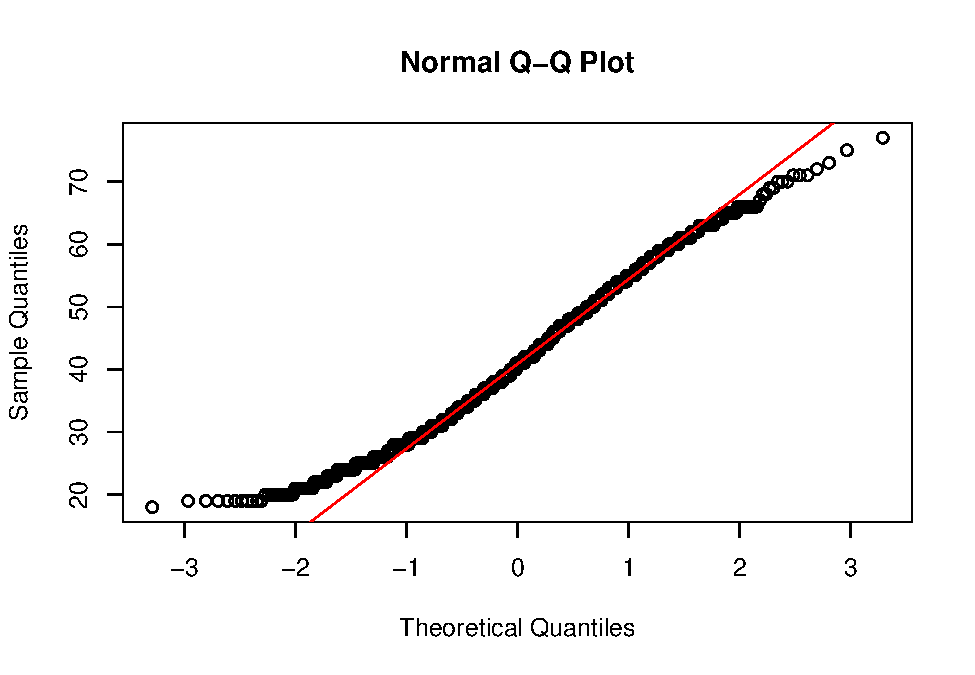
\includegraphics{C:/Users/DELL/OneDrive/R/Rprojetos/ufpr_ppgecon/estatistica/output/Exerc_1-Descritiva_alceunascimento_20240418_files/figure-latex/label, options-1.pdf}

\begin{Shaded}
\begin{Highlighting}[]
\FunctionTok{qqnorm}\NormalTok{(df1}\SpecialCharTok{$}\NormalTok{renda)}
\FunctionTok{qqline}\NormalTok{(df1}\SpecialCharTok{$}\NormalTok{renda, }\AttributeTok{col =} \StringTok{"red"}\NormalTok{)}
\end{Highlighting}
\end{Shaded}

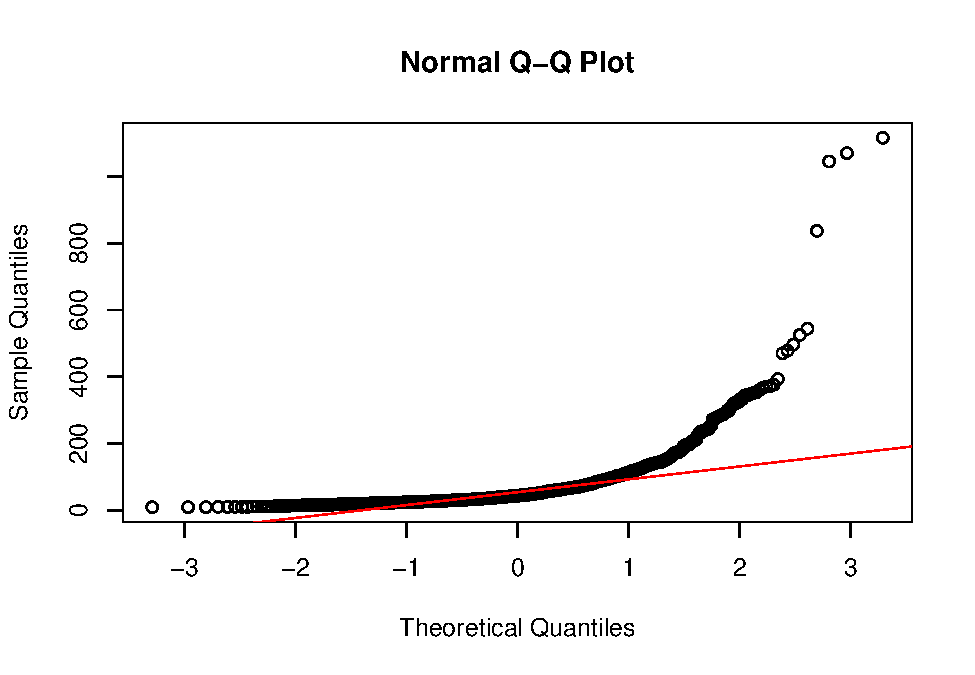
\includegraphics{C:/Users/DELL/OneDrive/R/Rprojetos/ufpr_ppgecon/estatistica/output/Exerc_1-Descritiva_alceunascimento_20240418_files/figure-latex/label, options-2.pdf}

\begin{Shaded}
\begin{Highlighting}[]
\FunctionTok{hist}\NormalTok{(df1}\SpecialCharTok{$}\NormalTok{idade, }\AttributeTok{probability =} \ConstantTok{TRUE}\NormalTok{, }\AttributeTok{main =} \StringTok{"Histograma com Curva de Densidade"}\NormalTok{)}
\FunctionTok{curve}\NormalTok{(}\FunctionTok{dnorm}\NormalTok{(x, }\AttributeTok{mean =} \FunctionTok{mean}\NormalTok{(df1}\SpecialCharTok{$}\NormalTok{idade), }\AttributeTok{sd =} \FunctionTok{sd}\NormalTok{(df1}\SpecialCharTok{$}\NormalTok{idade)), }
      \AttributeTok{add =} \ConstantTok{TRUE}\NormalTok{, }\AttributeTok{col =} \StringTok{"red"}\NormalTok{, }\AttributeTok{lwd =} \DecValTok{2}\NormalTok{)}
\end{Highlighting}
\end{Shaded}

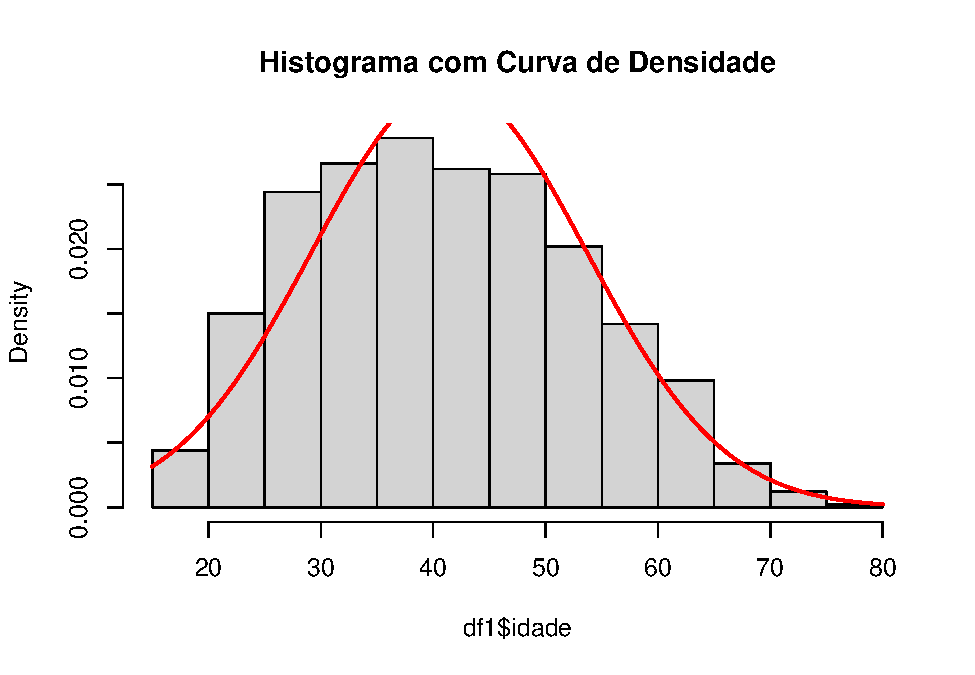
\includegraphics{C:/Users/DELL/OneDrive/R/Rprojetos/ufpr_ppgecon/estatistica/output/Exerc_1-Descritiva_alceunascimento_20240418_files/figure-latex/label, options-3.pdf}

\begin{Shaded}
\begin{Highlighting}[]
\FunctionTok{hist}\NormalTok{(df1}\SpecialCharTok{$}\NormalTok{renda, }\AttributeTok{probability =} \ConstantTok{TRUE}\NormalTok{, }\AttributeTok{main =} \StringTok{"Histograma com Curva de Densidade"}\NormalTok{)}
\FunctionTok{curve}\NormalTok{(}\FunctionTok{dnorm}\NormalTok{(x, }\AttributeTok{mean =} \FunctionTok{mean}\NormalTok{(df1}\SpecialCharTok{$}\NormalTok{renda), }\AttributeTok{sd =} \FunctionTok{sd}\NormalTok{(df1}\SpecialCharTok{$}\NormalTok{renda)), }
      \AttributeTok{add =} \ConstantTok{TRUE}\NormalTok{, }\AttributeTok{col =} \StringTok{"red"}\NormalTok{, }\AttributeTok{lwd =} \DecValTok{2}\NormalTok{)}
\end{Highlighting}
\end{Shaded}

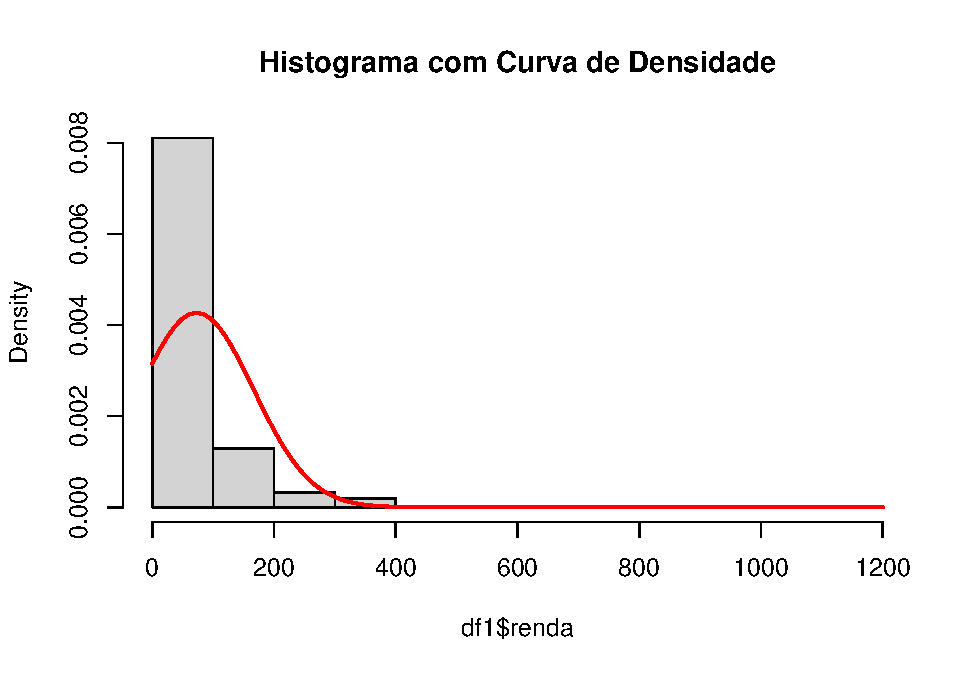
\includegraphics{C:/Users/DELL/OneDrive/R/Rprojetos/ufpr_ppgecon/estatistica/output/Exerc_1-Descritiva_alceunascimento_20240418_files/figure-latex/label, options-4.pdf}

\begin{Shaded}
\begin{Highlighting}[]
\CommentTok{\# Função para criar um gráfico Q{-}Q com ggplot2}
\NormalTok{make\_qqplot }\OtherTok{\textless{}{-}} \ControlFlowTok{function}\NormalTok{(data, var\_name) \{}
  \FunctionTok{ggplot}\NormalTok{(data, }\FunctionTok{aes}\NormalTok{(}\AttributeTok{sample =}\NormalTok{ .data[[var\_name]])) }\SpecialCharTok{+}
    \FunctionTok{stat\_qq}\NormalTok{() }\SpecialCharTok{+}
    \FunctionTok{stat\_qq\_line}\NormalTok{(}\AttributeTok{colour =} \StringTok{"red"}\NormalTok{) }\SpecialCharTok{+}
    \FunctionTok{ggtitle}\NormalTok{(}\FunctionTok{paste}\NormalTok{(}\StringTok{"Q{-}Q Plot de"}\NormalTok{, var\_name)) }\SpecialCharTok{+}
    \FunctionTok{theme\_minimal}\NormalTok{()}
\NormalTok{\}}

\CommentTok{\# Lista de variáveis numéricas (excluindo variáveis categóricas)}
\NormalTok{var\_names }\OtherTok{\textless{}{-}} \FunctionTok{c}\NormalTok{(}\StringTok{"idade"}\NormalTok{, }\StringTok{"renda"}\NormalTok{, }\StringTok{"carro"}\NormalTok{, }\StringTok{"t\_empr\_atual"}\NormalTok{)}

\CommentTok{\# Criar uma lista de gráficos Q{-}Q para cada variável}
\NormalTok{plots }\OtherTok{\textless{}{-}} \FunctionTok{lapply}\NormalTok{(var\_names, }\ControlFlowTok{function}\NormalTok{(v) }\FunctionTok{make\_qqplot}\NormalTok{(df1, v))}

\CommentTok{\# Organizar os gráficos em uma grade de 2 colunas}
\FunctionTok{grid.arrange}\NormalTok{(}\AttributeTok{grobs =}\NormalTok{ plots, }\AttributeTok{ncol =} \DecValTok{2}\NormalTok{)}
\end{Highlighting}
\end{Shaded}

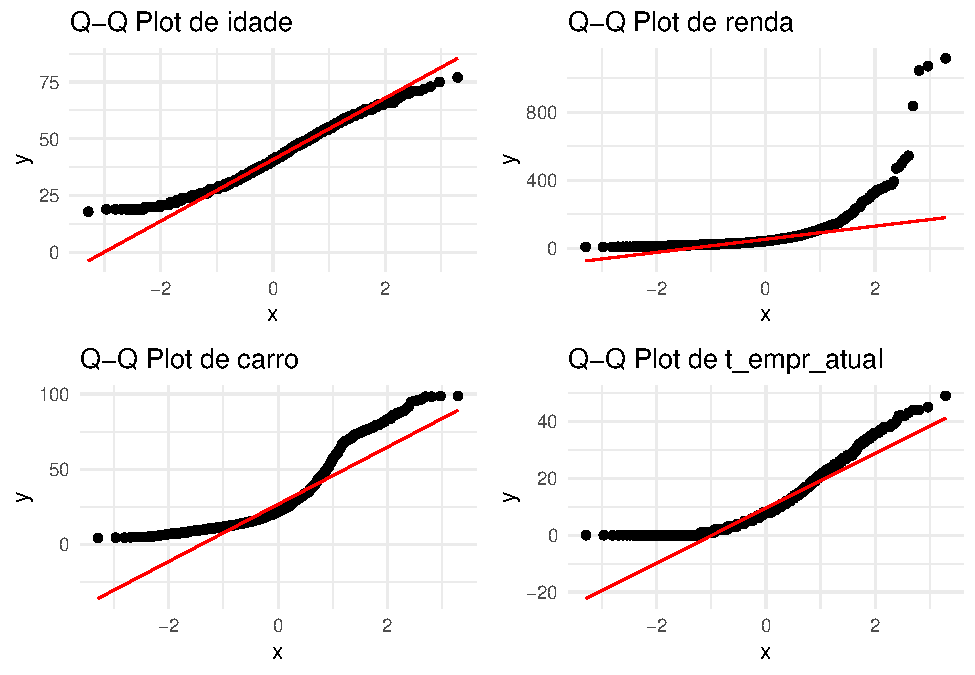
\includegraphics{C:/Users/DELL/OneDrive/R/Rprojetos/ufpr_ppgecon/estatistica/output/Exerc_1-Descritiva_alceunascimento_20240418_files/figure-latex/qq grid, options-1.pdf}

\begin{Shaded}
\begin{Highlighting}[]
\CommentTok{\# Função para criar um histograma com curva de densidade}
\NormalTok{make\_histogram }\OtherTok{\textless{}{-}} \ControlFlowTok{function}\NormalTok{(data, var\_name) \{}
  \CommentTok{\# Verifica se a variável é numérica; caso contrário, retorna NULL}
  \ControlFlowTok{if}\NormalTok{ (}\SpecialCharTok{!}\FunctionTok{is.numeric}\NormalTok{(data[[var\_name]])) \{}
    \FunctionTok{return}\NormalTok{(}\ConstantTok{NULL}\NormalTok{)}
\NormalTok{  \}}
  
\NormalTok{  p }\OtherTok{\textless{}{-}} \FunctionTok{ggplot}\NormalTok{(data, }\FunctionTok{aes\_string}\NormalTok{(}\AttributeTok{x =}\NormalTok{ var\_name)) }\SpecialCharTok{+}
    \FunctionTok{geom\_histogram}\NormalTok{(}\FunctionTok{aes}\NormalTok{(}\AttributeTok{y =}\NormalTok{ ..density..), }\AttributeTok{bins =} \DecValTok{30}\NormalTok{, }\AttributeTok{fill =} \StringTok{"gray"}\NormalTok{, }\AttributeTok{alpha =} \FloatTok{0.7}\NormalTok{) }\SpecialCharTok{+}
    \FunctionTok{geom\_density}\NormalTok{(}\AttributeTok{color =} \StringTok{"red"}\NormalTok{, }\AttributeTok{size =} \FloatTok{1.5}\NormalTok{) }\SpecialCharTok{+}
    \FunctionTok{labs}\NormalTok{(}\AttributeTok{title =} \FunctionTok{paste}\NormalTok{(}\StringTok{"Histograma com Curva de Densidade {-}"}\NormalTok{, var\_name),}
         \AttributeTok{x =}\NormalTok{ var\_name,}
         \AttributeTok{y =} \StringTok{"Densidade"}\NormalTok{) }\SpecialCharTok{+}
    \FunctionTok{theme\_minimal}\NormalTok{()}
  \FunctionTok{return}\NormalTok{(p)}
\NormalTok{\}}

\CommentTok{\# Lista de variáveis numéricas}
\NormalTok{var\_names }\OtherTok{\textless{}{-}} \FunctionTok{c}\NormalTok{(}\StringTok{"idade"}\NormalTok{, }\StringTok{"renda"}\NormalTok{, }\StringTok{"carro"}\NormalTok{, }\StringTok{"t\_empr\_atual"}\NormalTok{)  }

\CommentTok{\# Criar uma lista de gráficos para cada variável numérica}
\NormalTok{plots }\OtherTok{\textless{}{-}} \FunctionTok{lapply}\NormalTok{(var\_names, }\ControlFlowTok{function}\NormalTok{(v) }\FunctionTok{make\_histogram}\NormalTok{(df1, v))}
\NormalTok{plots }\OtherTok{\textless{}{-}}\NormalTok{ plots[}\SpecialCharTok{!}\FunctionTok{sapply}\NormalTok{(plots, is.null)]  }\CommentTok{\# Remove NULLs caso alguma variável não seja numérica}

\CommentTok{\# Organizar os gráficos em uma grade de 2 colunas}
\FunctionTok{grid.arrange}\NormalTok{(}\AttributeTok{grobs =}\NormalTok{ plots, }\AttributeTok{ncol =} \DecValTok{2}\NormalTok{)}
\end{Highlighting}
\end{Shaded}

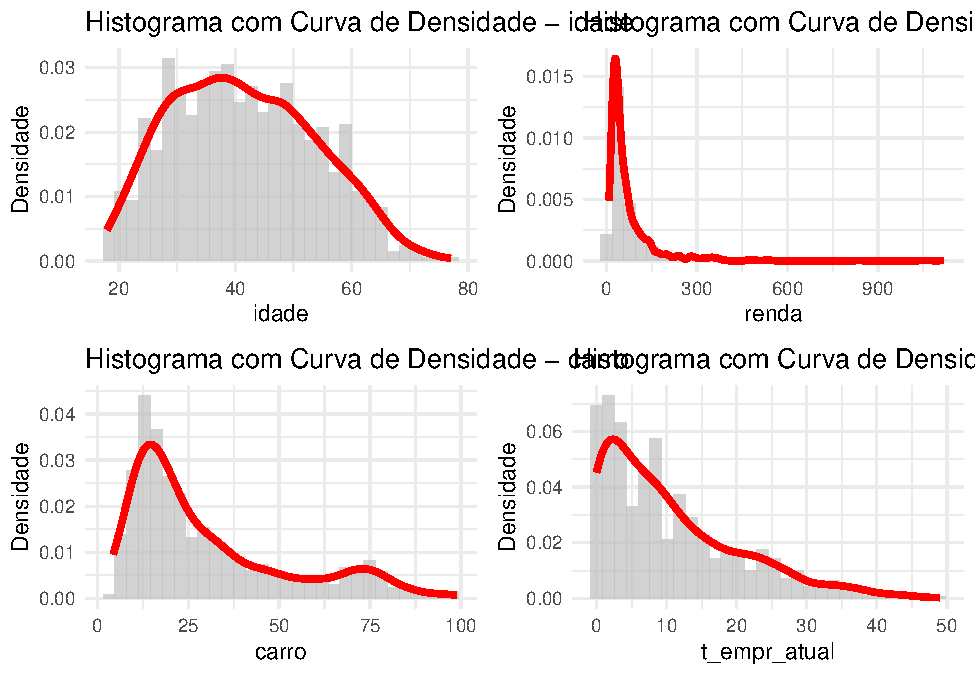
\includegraphics{C:/Users/DELL/OneDrive/R/Rprojetos/ufpr_ppgecon/estatistica/output/Exerc_1-Descritiva_alceunascimento_20240418_files/figure-latex/hist grid, options-1.pdf}

\hypertarget{item-2-dataset-2}{%
\subsection{Item 2 (dataset 2)}\label{item-2-dataset-2}}

Ao lado são apresentados dados de gastos per capita, em milhares de
dólares, para cada estado americano em 20xx.

\hypertarget{apurauxe7uxe3o-1}{%
\subsubsection{APURAÇÃO}\label{apurauxe7uxe3o-1}}

\begin{Shaded}
\begin{Highlighting}[]
\NormalTok{df2 }\OtherTok{\textless{}{-}} \FunctionTok{read\_csv2}\NormalTok{(}\StringTok{"C:/Users/DELL/OneDrive/R/Rprojetos/ufpr\_ppgecon/estatistica/data/Exerc\_1\_descritiva\_dataset2.csv"}\NormalTok{)}
\end{Highlighting}
\end{Shaded}

\begin{verbatim}
## i Using "','" as decimal and "'.'" as grouping mark. Use `read_delim()` for more control.
\end{verbatim}

\begin{verbatim}
## Rows: 50 Columns: 2
## -- Column specification -------------------------------------------------------------------------------------------------------------------------------
## Delimiter: ";"
## chr (1): estado
## dbl (1): gasto
## 
## i Use `spec()` to retrieve the full column specification for this data.
## i Specify the column types or set `show_col_types = FALSE` to quiet this message.
\end{verbatim}

\begin{Shaded}
\begin{Highlighting}[]
\NormalTok{df2}
\end{Highlighting}
\end{Shaded}

\begin{verbatim}
## # A tibble: 50 x 2
##    estado      gasto
##    <chr>       <dbl>
##  1 Alabama      8.62
##  2 Alasca      12.9 
##  3 Arizona      7.31
##  4 Arkansas     7.08
##  5 Califórnia   6.47
##  6 Colorado     6.53
##  7 Connecticut  8.65
##  8 Delaware     6.33
##  9 Flórida      7.01
## 10 Georgia      6.25
## # i 40 more rows
\end{verbatim}

\begin{Shaded}
\begin{Highlighting}[]
\FunctionTok{summary}\NormalTok{(df2)}
\end{Highlighting}
\end{Shaded}

\begin{verbatim}
##     estado              gasto         
##  Length:50          Min.   : 5.46900  
##  Class :character   1st Qu.: 6.36175  
##  Mode  :character   Median : 7.26300  
##                     Mean   : 7.52730  
##                     3rd Qu.: 8.20725  
##                     Max.   :12.88500
\end{verbatim}

\hypertarget{questuxf5es-1}{%
\subsubsection{QUESTÕES:}\label{questuxf5es-1}}

\begin{enumerate}
\def\labelenumi{\alph{enumi})}
\tightlist
\item
  Faça um resumo das estatísticas descritivas desses dados\\
\item
  Decida se os dados apresentados podem estar aproximadamente
  normalmente distribuídos
\end{enumerate}

\hypertarget{item-3}{%
\subsection{Item 3}\label{item-3}}

Suponha que o volume de negócios diários comercializados na Bolsa de
Nova York (NYSE) seja uma variável normalmente distribuída com média de
1,8 bilhão e desvio-padrão de 0,15 bilhão.

\hypertarget{apurauxe7uxe3o-2}{%
\subsubsection{APURAÇÃO}\label{apurauxe7uxe3o-2}}

\begin{Shaded}
\begin{Highlighting}[]
\CommentTok{\# parametros}
\NormalTok{mean3 }\OtherTok{\textless{}{-}} \FloatTok{1.8}
\NormalTok{sd3 }\OtherTok{\textless{}{-}} \FloatTok{0.15}
\end{Highlighting}
\end{Shaded}

\begin{Shaded}
\begin{Highlighting}[]
\CommentTok{\# Calculando as probabilidades }
\DocumentationTok{\#\# Usando \textquotesingle{}pnorm\textquotesingle{}: probabilidade de ser menor ou igual a um valor (dist normal)}
\NormalTok{prob\_a }\OtherTok{\textless{}{-}} \FunctionTok{pnorm}\NormalTok{(}\FloatTok{1.5}\NormalTok{, }\AttributeTok{mean =}\NormalTok{ mean3, }\AttributeTok{sd =}\NormalTok{ sd3)}
\NormalTok{prob\_b }\OtherTok{\textless{}{-}} \DecValTok{1} \SpecialCharTok{{-}} \FunctionTok{pnorm}\NormalTok{(}\DecValTok{2}\NormalTok{, }\AttributeTok{mean =}\NormalTok{ mean3, }\AttributeTok{sd =}\NormalTok{ sd3)}
\NormalTok{prob\_c }\OtherTok{\textless{}{-}} \FunctionTok{pnorm}\NormalTok{(}\FloatTok{1.9}\NormalTok{, }\AttributeTok{mean =}\NormalTok{ mean3, }\AttributeTok{sd =}\NormalTok{ sd3) }\SpecialCharTok{{-}} \FunctionTok{pnorm}\NormalTok{(}\FloatTok{1.7}\NormalTok{, }\AttributeTok{mean =}\NormalTok{ mean3, }\AttributeTok{sd =}\NormalTok{ sd3)}

\CommentTok{\# Gerando um gráfico}
\DocumentationTok{\#\# Criando um data frame para o gráfico}
\NormalTok{x }\OtherTok{\textless{}{-}} \FunctionTok{seq}\NormalTok{(mean3 }\SpecialCharTok{{-}} \DecValTok{4}\SpecialCharTok{*}\NormalTok{sd3, mean3 }\SpecialCharTok{+} \DecValTok{5}\SpecialCharTok{*}\NormalTok{sd3, }\AttributeTok{length.out =} \DecValTok{1000}\NormalTok{)}
\NormalTok{y }\OtherTok{\textless{}{-}} \FunctionTok{dnorm}\NormalTok{(x, }\AttributeTok{mean =}\NormalTok{ mean3, }\AttributeTok{sd =}\NormalTok{ sd3)}
\NormalTok{data }\OtherTok{\textless{}{-}} \FunctionTok{data.frame}\NormalTok{(x, y)}

\DocumentationTok{\#\# Gerando o gráfico}
\FunctionTok{ggplot}\NormalTok{(data, }\FunctionTok{aes}\NormalTok{(x, y)) }\SpecialCharTok{+}
  \FunctionTok{geom\_line}\NormalTok{() }\SpecialCharTok{+}
  \FunctionTok{stat\_function}\NormalTok{(}
    \AttributeTok{fun =}\NormalTok{ dnorm, }
    \AttributeTok{args =} \FunctionTok{list}\NormalTok{(}\AttributeTok{mean =}\NormalTok{ mean3, }\AttributeTok{sd =}\NormalTok{ sd3), }
    \AttributeTok{geom =} \StringTok{"area"}\NormalTok{, }
    \AttributeTok{fill =} \StringTok{"blue"}\NormalTok{, }
    \AttributeTok{xlim =} \FunctionTok{c}\NormalTok{(}\DecValTok{1}\NormalTok{, }\FloatTok{1.5}\NormalTok{), }
    \AttributeTok{alpha =} \FloatTok{0.3}\NormalTok{) }\SpecialCharTok{+}
  \FunctionTok{stat\_function}\NormalTok{(}
    \AttributeTok{fun =}\NormalTok{ dnorm, }
    \AttributeTok{args =} \FunctionTok{list}\NormalTok{(}\AttributeTok{mean =}\NormalTok{ mean3, }\AttributeTok{sd =}\NormalTok{ sd3), }
    \AttributeTok{geom =} \StringTok{"area"}\NormalTok{, }
    \AttributeTok{fill =} \StringTok{"red"}\NormalTok{, }
    \AttributeTok{xlim =} \FunctionTok{c}\NormalTok{(}\DecValTok{2}\NormalTok{, }\FloatTok{2.5}\NormalTok{), }
    \AttributeTok{alpha =} \FloatTok{0.3}\NormalTok{) }\SpecialCharTok{+}
  \FunctionTok{stat\_function}\NormalTok{(}
    \AttributeTok{fun =}\NormalTok{ dnorm, }
    \AttributeTok{args =} \FunctionTok{list}\NormalTok{(}\AttributeTok{mean =}\NormalTok{ mean3, }\AttributeTok{sd =}\NormalTok{ sd3), }
    \AttributeTok{geom =} \StringTok{"area"}\NormalTok{, }
    \AttributeTok{fill =} \StringTok{"green"}\NormalTok{, }
    \AttributeTok{xlim =} \FunctionTok{c}\NormalTok{(}\FloatTok{1.7}\NormalTok{, }\FloatTok{1.9}\NormalTok{), }
    \AttributeTok{alpha =} \FloatTok{0.3}\NormalTok{) }\SpecialCharTok{+}
  \FunctionTok{labs}\NormalTok{(}\AttributeTok{title =} \StringTok{\textquotesingle{}Volume de Negócios na NYSE\textquotesingle{}}\NormalTok{,}
       \AttributeTok{subtitle =} \StringTok{\textquotesingle{}Assumindo uma distribuição normal\textquotesingle{}}\NormalTok{,}
       \AttributeTok{x =} \StringTok{\textquotesingle{}Volume de Negócios (bilhões)\textquotesingle{}}\NormalTok{,}
       \AttributeTok{y =} \StringTok{\textquotesingle{}Probabilidade\textquotesingle{}}\NormalTok{) }\SpecialCharTok{+}
  \FunctionTok{theme\_bw}\NormalTok{()}
\end{Highlighting}
\end{Shaded}

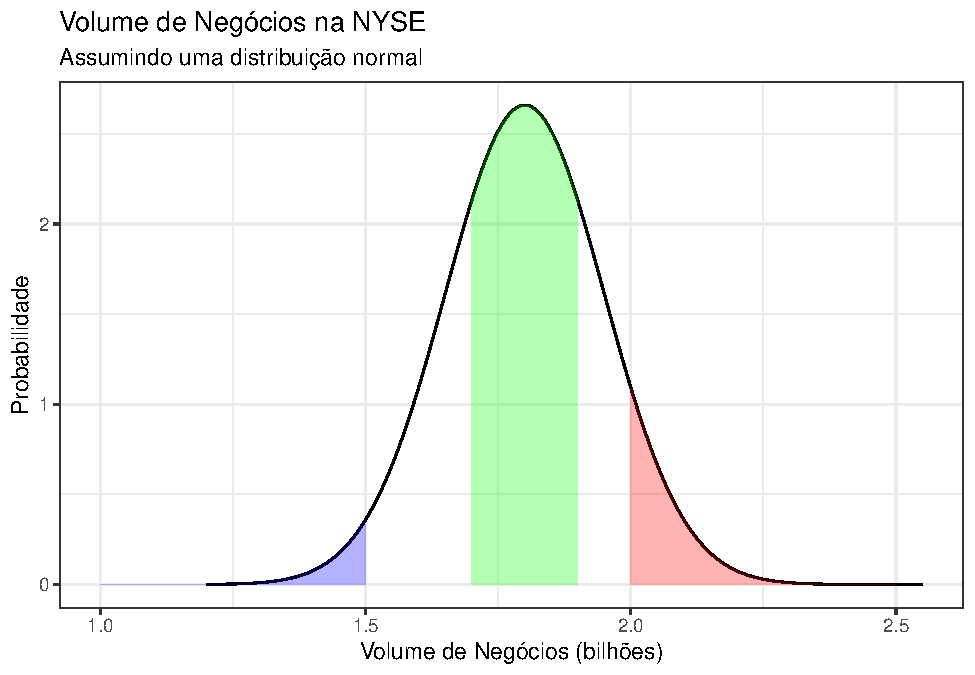
\includegraphics{C:/Users/DELL/OneDrive/R/Rprojetos/ufpr_ppgecon/estatistica/output/Exerc_1-Descritiva_alceunascimento_20240418_files/figure-latex/analize data 3, options-1.pdf}

\hypertarget{questuxf5es-2}{%
\subsubsection{QUESTÕES:}\label{questuxf5es-2}}

Para um dia aleatoriamente escolhido, qual a probabilidade do volume
estar:\\
a) abaixo de 1,5 bilhão?\\
Resp: 0.0227501319\\
b) acima de 2 bilhões?\\
Resp: 0.0912112197\\
c) entre 1,7 e 1,9 bilhão?\\
Resp: 0.4950149249

\hypertarget{item-4}{%
\subsection{Item 4}\label{item-4}}

Uma análise estatística de 1.000 chamadas telefônicas de longa distância
originadas dos escritórios da Bricks and Clicks Computer Corporation
indicam que a duração dessas chamadas estão normalmente distribuídas.
Sendo a média e o desvio-padrão da duração das chamadas 240 segundos e
40 segundos, respectivamente.

\hypertarget{apurauxe7uxe3o-3}{%
\subsubsection{APURAÇÃO}\label{apurauxe7uxe3o-3}}

\begin{Shaded}
\begin{Highlighting}[]
\NormalTok{mean4 }\OtherTok{\textless{}{-}} \DecValTok{240}
\NormalTok{sd4 }\OtherTok{\textless{}{-}} \DecValTok{40}
\end{Highlighting}
\end{Shaded}

\hypertarget{questuxf5es-3}{%
\subsubsection{QUESTÕES:}\label{questuxf5es-3}}

\begin{enumerate}
\def\labelenumi{\alph{enumi})}
\tightlist
\item
  Calcule a probabilidade de uma chamada durar menos de 180 segundos.\\
\item
  Qual a probabilidade de uma chamada durar entre 200 e 300 segundos?\\
\item
  Um empregado realizou diversas chamadas com duração acima de 350
  segundos.\\
  Você pode aceitar que esse é um fato casual?
\end{enumerate}

\hypertarget{item-5-dataset-5}{%
\subsection{Item 5 (dataset 5)}\label{item-5-dataset-5}}

Uma pesquisa realizada entre instituições financeiras da América Latina
apresentou os resultados descritos na tabela abaixo. Você diria que
existe associação entre o tempo de atuação e o número de clientes?

\hypertarget{apurauxe7uxe3o-4}{%
\subsubsection{APURAÇÃO}\label{apurauxe7uxe3o-4}}

\begin{Shaded}
\begin{Highlighting}[]
\NormalTok{df5 }\OtherTok{\textless{}{-}} \FunctionTok{read\_csv2}\NormalTok{(}\StringTok{"C:/Users/DELL/OneDrive/R/Rprojetos/ufpr\_ppgecon/estatistica/data/Exerc\_1\_descritiva\_dataset5.csv"}\NormalTok{)}
\end{Highlighting}
\end{Shaded}

\begin{verbatim}
## i Using "','" as decimal and "'.'" as grouping mark. Use `read_delim()` for more control.
\end{verbatim}

\begin{verbatim}
## Rows: 5 Columns: 3
## -- Column specification -------------------------------------------------------------------------------------------------------------------------------
## Delimiter: ";"
## chr (1): Instituição
## dbl (2): Tempo de atuação, Número de clientes
## 
## i Use `spec()` to retrieve the full column specification for this data.
## i Specify the column types or set `show_col_types = FALSE` to quiet this message.
\end{verbatim}

\begin{Shaded}
\begin{Highlighting}[]
\NormalTok{df5}
\end{Highlighting}
\end{Shaded}

\begin{verbatim}
## # A tibble: 5 x 3
##   Instituição `Tempo de atuação` `Número de clientes`
##   <chr>                    <dbl>                <dbl>
## 1 A                           25                  102
## 2 B                           32                  121
## 3 C                           28                   80
## 4 D                           53                  181
## 5 E                           44                  132
\end{verbatim}

\hypertarget{questuxf5es-4}{%
\subsubsection{QUESTÕES:}\label{questuxf5es-4}}

\begin{enumerate}
\def\labelenumi{\alph{enumi})}
\tightlist
\item
  Construa o diagrama de dispersão dos dados.\\
\item
  Calcule a covariância e o coeficiente de correlação.
\end{enumerate}

\hypertarget{item-6-dataset-6}{%
\subsection{Item 6 (dataset 6)}\label{item-6-dataset-6}}

Os preços de fechamento de diversos ativos negociados na BOVESPA
aparecem listados na planilha portfolio.

\hypertarget{apurauxe7uxe3o-5}{%
\subsubsection{APURAÇÃO}\label{apurauxe7uxe3o-5}}

\begin{Shaded}
\begin{Highlighting}[]
\NormalTok{df6 }\OtherTok{\textless{}{-}} \FunctionTok{read\_csv2}\NormalTok{(}\StringTok{"C:/Users/DELL/OneDrive/R/Rprojetos/ufpr\_ppgecon/estatistica/data/Exerc\_1\_descritiva\_dataset6.csv"}\NormalTok{)}
\end{Highlighting}
\end{Shaded}

\begin{verbatim}
## i Using "','" as decimal and "'.'" as grouping mark. Use `read_delim()` for more control.
\end{verbatim}

\begin{verbatim}
## Rows: 599 Columns: 15
## -- Column specification -------------------------------------------------------------------------------------------------------------------------------
## Delimiter: ";"
## chr  (1): date
## dbl (14): PETR4, VALE5, CSNA3, GGBR4, USIM5, JBSS3, MRFG3, BEEF3, LAME4, AMBV4, NATU3, ITUB4, BBDC4, BBAS3
## 
## i Use `spec()` to retrieve the full column specification for this data.
## i Specify the column types or set `show_col_types = FALSE` to quiet this message.
\end{verbatim}

\begin{Shaded}
\begin{Highlighting}[]
\NormalTok{df6}
\end{Highlighting}
\end{Shaded}

\begin{verbatim}
## # A tibble: 599 x 15
##    date       PETR4 VALE5 CSNA3 GGBR4 USIM5 JBSS3 MRFG3 BEEF3 LAME4 AMBV4 NATU3 ITUB4 BBDC4 BBAS3
##    <chr>      <dbl> <dbl> <dbl> <dbl> <dbl> <dbl> <dbl> <dbl> <dbl> <dbl> <dbl> <dbl> <dbl> <dbl>
##  1 20/05/2008  47.2  54.1  37.7  40.0  42.6  8.31  20.2  10.3  12.8  117.  18.3  32.3  30.4  25.9
##  2 21/05/2008  48.0  52.6  36.7  38.9  41.1  8.56  20.5  10.2  12.5  114.  17.2  31.5  29.7  25.1
##  3 23/05/2008  46.2  51.9  36.7  38.6  41.0  8.46  20.6   9.8  12.5  111.  16.6  31.4  29.7  24.4
##  4 26/05/2008  47.1  51.6  37.1  39.1  41.3  8.42  20.8  10.1  12.5  111.  16.7  31.4  29.3  24.4
##  5 27/05/2008  45.6  50.5  36.5  39.2  40.5  8.61  21.4  10.3  12.2  110.  16.4  32.3  29.9  25.0
##  6 28/05/2008  46.6  51.6  37.6  40.1  41.4  9.26  22.6  10.6  12.6  107.  17.2  33.4  31.0  26.5
##  7 29/05/2008  45.1  49.3  36.2  38.5  40.4  9.64  22.5  10.8  12.8  105.  17.7  33.2  30.4  26.7
##  8 30/05/2008  44.8  50.2  35.6  39.0  40.5  9.84  23.0  11.2  12.9  105.  17.1  34.5  30.9  28.0
##  9 02/06/2008  45.5  50.2  35.5  38.5  40.2  9.64  22.5  11.2  12.4  103.  16.7  33.0  30.2  27.2
## 10 03/06/2008  43.3  48.5  34.6  38.3  39.8  9.13  22.7  11.3  12.5  100.  16.5  32.1  29.5  26.2
## # i 589 more rows
\end{verbatim}

\hypertarget{questuxf5es-5}{%
\subsubsection{QUESTÕES:}\label{questuxf5es-5}}

\begin{enumerate}
\def\labelenumi{\alph{enumi})}
\tightlist
\item
  Se você fosse comprar somente um dos papéis dentre os listados, qual
  seria a melhor escolha com base no período analisado?\\
\item
  Calcule o risco e o retorno de uma carteira formada com 50\% de PETR4
  e 50\% de VALE5. Simule o resultado para diversos níveis de
  correlação.\\
\item
  Encontre os papéis com menor correlação.\\
\item
  Com base nesses dois papéis, qual percentual do seu capital você
  aplicaria em cada ação para obter a carteira de menor risco?\\
\item
  Os retornos parecem seguir uma curva normal?
\end{enumerate}

\end{document}
